\documentclass{article}

\usepackage[utf8]{inputenc}
\usepackage[russian]{babel}
\usepackage[a4paper, margin=1in]{geometry}
\usepackage{graphicx}
\usepackage{amsmath}
\usepackage{wrapfig}
\usepackage{multirow}
\usepackage{mathtools}
\usepackage{pgfplots}
\usepackage{pgfplotstable}
\usepackage{setspace}
\usepackage{changepage}
\usepackage{caption}
\usepackage{csquotes}
\usepackage{hyperref}
\usepackage{listings}
\usepackage{subfigure}
\usepackage{float}

\pgfplotsset{compat=1.18}
\hypersetup{
  colorlinks = true,
  linkcolor  = blue,
  filecolor  = magenta,      
  urlcolor   = darkgray,
  pdftitle   = mobile-smarthouse-report,
}

\definecolor{codegreen}{rgb}{0,0.6,0}
\definecolor{codegray}{rgb}{0.5,0.5,0.5}
\definecolor{codepurple}{rgb}{0.58,0,0.82}
\definecolor{backcolour}{rgb}{0.99,0.99,0.99}

\lstdefinestyle{codestyle}{
  backgroundcolor=\color{backcolour},   
  commentstyle=\color{codegreen},
  keywordstyle=\color{magenta},
  numberstyle=\tiny\color{codegray},
  stringstyle=\color{codepurple},
  basicstyle=\ttfamily\footnotesize,
  breakatwhitespace=false,         
  breaklines=true,                 
  captionpos=b,                    
  keepspaces=true,                 
  numbers=left,                    
  numbersep=5pt,                  
  showspaces=false,                
  showstringspaces=false,
  showtabs=false,                  
  tabsize=2
}

\lstset{style=codestyle}

\begin{document}

\begin{titlepage}
\centering{\vspace*{0.4cm}
\includegraphics[height=2.5cm]{images/ITMO_University_logo.png}}
    \begin{center}
        \begin{spacing}{1.4}
            \large{Университет ИТМО} \\
            \large{Факультет программной инженерии и компьютерной техники} \\
        \end{spacing}
        \vfill
        \textbf{
            \huge{Разработка мобильных приложений} \\
            \huge{Проект SmartHouse} \\
        }
    \end{center}
    \vfill
    \begin{center}
        \begin{tabular}{r l}
            Студенты:       & Гиниятуллин Арслан Рафаилович P33121 \\
                            & Сущенко Роман Витальевич P33131 \\
                            & Гиря Максим Дмитриевич P33131 \\
                            & Тороев Канатбек Бакытбекович P33131 \\
            Преподаватель:  & Ключев Аркадий Олегович \\
        \end{tabular}
    \end{center}
    \vfill
    \begin{center}
        \begin{large}
            2024
        \end{large}
    \end{center}
\end{titlepage}


\tableofcontents

\section{Введение}

Система умного дома \textbf{SmartHouse} представляет собой комплекс технологических решений, направленных на обеспечение комфорта, безопасности и энергоэффективности в современном жилище. В последнее десятилетие интерес к умным домам значительно возрос благодаря развитию Интернета вещей \textit{(IoT)}, усовершенствованию беспроводных технологий и доступности интеллектуальных устройств. 

\subsection{Актуальность работы}
    Современный образ жизни ставит перед нами множество задач, требующих эффективного использования времени и ресурсов. В условиях урбанизации и нескончаемых деловых обязанностей важно обеспечить максимальный комфорт и безопасность в доме при минимальных усилиях. Система \textbf{SmartHouse} предоставляет возможность автоматизации повседневных операций и задач, таких как управление освещением, климат-контролем, охраной и множеством других бытовых процессов. Крупные компании \textit{(Яндекс, Сбер Девайсы, Apple, Xiaomi)} уже заметили этот рынок и предлагают свои решения: \textit{Умный дом с Алисой, Xiaomi Mi Home}. \\ \\
Актуальность системы умного дома подтверждается следующими аргументами:

\begin{enumerate}
     \item \textbf{Рост числа подключенных устройств:} По данным аналитических компаний, количество IoT-устройств в мире продолжает стремительно расти, и к 2025 году их число превысит 75 миллиардов. Умные дома становятся частью повседневной жизни, интегрируя множество устройств в единую управляемую систему.
     
    \item \textbf{Повышенные требования к безопасности:} С увеличением тревожности по поводу безопасности жилья возрастает спрос на системы видеонаблюдения, сигнализации и датчиков утечки. \textbf{SmartHouse} обеспечивает многоуровневую защиту, помогая пользователям чувствовать себя в безопасности.
   
    \item \textbf{Энергоэффективность и экологическая осознанность:} В условиях роста стоимости энергоресурсов и изменения климата становится все более важным снижать энергопотребление. Система умного дома позволяет оптимизировать использование энергии, экономя ресурсы и снижая экологический след.
   
    \item \textbf{Высокие ожидания потребителей:} Современные пользователи уже привыкли к удобству и простоте использования интеллектуальных устройств. Они ожидают, что дом также станет "умным", предоставляя функции автоматизированного управления освещением, климатом, безопасностью и другими аспектами быта.
   
    \item \textbf{Удобство и качество жизни:} Современные решения для умного дома не только делают жизнь удобнее, но и улучшают ее качество. Автоматизация рутинных задач освобождает время для более важных дел и повышения общего уровня комфорта.

    \item \textbf{Развитие экосистем:} Интеграция с платформами таких крупных игроков рынка, как \textit{Google Home, Apple HomeKit и Amazon Alexa, Яндекс Алиса} делает управление домом более удобным и функциональным.

\end{enumerate}


\subsection{Цель работы}

Основная цель разработки и внедрения системы умного дома \textbf{SmartHouse} - это создание комфортной, безопасной и энергоэффективной среды проживания. Данная цель достигается за счет использования современных технологий и интеграции различных интеллектуальных устройств в единую управляемую экосистему.

\subsection{Задачи}
Для достижения поставленной цели необходимо выполнить следующие задачи:

\begin{enumerate}
    
    \item \textbf{Разработка пользовательского приложения для управления умным домом:} Создать удобное и функциональное приложение, которое позволит пользователям максимально комфортно управлять различными интеллектуальными устройствами. Программное обеспечение должно обеспечивать интеграцию всех устройств и надежную работу системы, отвечая основной цели проекта создания комфортной и энергоэффективной среды проживания.

    \item \textbf{Изучение и выбор технологий и протоколов:} Провести анализ доступных технологий и протоколов, которые обеспечат наибольшую совместимость с широким спектром устройств. Это поддержит цель создания безопасной и энергоэффективной экосистемы умного дома, упрощая процесс внедрения для пользователей.

    \item \textbf{Разработка расширяемой и гибкой системы:} Обеспечить возможность легкого добавления новых устройств и функциональных возможностей без необходимости пересмотра всей системы. Это соответствует цели проекта по созданию удобной и комфортной среды, позволяя пользователям адаптировать умный дом под свои индивидуальные нужды и предпочтения.

    \item \textbf{Обеспечение безопасности и конфиденциальности:} Разработать и внедрить надежные механизмы защиты данных пользователей и системы от несанкционированного доступа. Эта задача непосредственно направлена на достижение цели создания безопасной среды проживания, гарантируя пользователям защиту их данных и устройств в системе умного дома.
\end{enumerate}

\section{Техническое задание}

\subsection{Введение}
В данном этапе представлено техническое задание на разработку \textit{IoT} системы \textbf{SmartHouse}, предназначенной для создание комфортной, безопасной и энергоэффективной среды проживания. Включены ключевые требования и спецификации, которые необходимо учесть в процессе разработки.

\subsection{Назначение разработки}
Цель разработки системы \textbf{SmartHouse} является обеспечение безопасности на территории завода путем реализации функций контроля и оповещения о несанкционированных проникновениях, пожарах, утечках воды и иных опасных ситуациях. Система также предназначена для мониторинга доступа в помещения и управления оперативными данными.


\subsection{Требования к программе или программному изделию}

\subsubsection{Функциональные требования}

\begin{table}[H]
    \centering
    \begin{tabular}{|c|p{10cm}|c|c|}
    \hline
        № & \centering Требования & Приоритет & Трудоемкость \\ \hline
        1 & Система пожарной сигнализации должна автоматически вызывать пожарных и отправлять уведомление пользователю (+ включать сигнализацию) при возгорании или задымлении в помещении (повышении температуры или уровня дыма) & must & 8 члвк/ час \\ \hline
        2 & Система должна обнаруживать и регистрировать движения в зоне видимости камер, сохраняя данные для удаленного доступа & must & 6 члвк/ час \\ \hline
        3 & Система интеграции с дверьми и окнами должна регистрировать (+ включать сигнализацию) несанкционированное проникновение и отправлять уведомление пользователю и/или вызывать полицию & must & 8 члвк/ час \\ \hline
        4 & Система должна предоставлять удаленный просмотр видео с камер наблюдения через приложение & must & 3 члвк/ час \\ \hline
        5 & Система может предоставлять автоматическое резервное копирование и восстановление для сохранения настроек системы безопасности и важной информации в случае сбоев & could & 5 члвк/ час \\ \hline
        6 & Система должна предоставлять защиту от протечек с возможностью автоматического перекрытия подачи воды и уведомлением пользователя при обнаружении утечки & must & 6 члвк/ час \\ \hline
        7 & Система должна предоставлять контроль доступа с использованием персональных кодов для безопасного и удобного входа и выхода из дома & must & 6 члвк/ час \\ \hline
    \end{tabular}
    \caption{Требования к безопасности системы SmartHouse}
\end{table}


\begin{table}[H]
    \centering
    \begin{tabular}{|c|p{7cm}|c|c|}
    \hline
        № & Требования & Приоритетность & Трудоемкость \\ \hline
        1 & Система должна позволять пользователю отслеживать потребление всех его датчиков & must & 8 члвк/ час \\ \hline
        2 & Система должна позволять пользователю настроить уведомление о высоком энергопотреблении & must & 8 члвк/ час \\ \hline
        3 & Система должна автоматически регулировать температуру в доме с помощью датчиков & must & 16 члвк/ час \\ \hline
        4 & Система должна переводить датчики в режим энергосбережения, или выключать их, если они не используются & could & 16 члвк/ час \\ \hline
        5 & Система должна автоматически регулировать включение или выключение света в зависимости от датчика движения & must & 8 члвк/ час\\ \hline
    \end{tabular}
        \caption{Требования к энергосбережению системы SmartHouse}
\end{table}


\begin{table}[H]
    \centering
    \begin{tabular}{|c|p{7cm}|c|c|}
    \hline
        № & Требования & Приоритетность & Трудоемкость \\ \hline
        1 & Система должна позволять пользователю создать аккаунт, указав электронную почту, пароль, персональные данные (ФИО, телефон) & must & 20 члвк/ час \\ \hline
        2 & Система должна позволять пользователю войти в аккаунт по логину+паролю & must & 20 члвк/ час \\ \hline
        3 & Система должна позволять пользователю изменить пароль при указании почты используя двуфакторную аунтификацию.  & could & 40 члвк/ час \\ \hline
        4 & Система должна позволять пользователю создать объект Семья, став при этом ее Владельцем & could & 30 члвк/час \\ \hline
        5 & Система должна позволять пользователю получить ссылку для приглашения нового участника в семью.     & could & 30 члвк/час \\ \hline
        6 & Система должна позволять пользователю добавить объект Комната в Дом, указав ее название.    & should & 10 члвк/час \\ \hline
        7 &  Система должна позволять пользователю включать/выключать Режим в Доме          & must & 15  члвк/час \\ \hline
        8 &  Система должна позволять пользователю включить/выключить Устройство в комнате.    & must & 10 члвк/час \\ \hline
        9 & Система должна позволять пользователю создать объект Комнатный Режим с указанием названия и набора Настроек Устройств находящихся в соответствующей Комнате.  & should & 15 члвк/час \\ \hline
        10 & Система должна позволять пользователю отображать/изменять текущую температуру в комнатах. & must & 30 члвк/час \\ \hline
    \end{tabular}
    \caption{Требования к комфорту системы SmartHouse}
\end{table}


\subsubsection{Нефункциональные требования}

\begin{table}[H]
    \centering
    \begin{tabular}{|c|c|p{7cm}|}
    \hline
        № & Требования & Описание \\ \hline
        1 & Производительность & Система должна выдерживать нагрузку 10 запросов в секунду (10 RPS). \\ \hline
        2 & Надежность & Система должна иметь механизмы для обеспечения высокой надежности, включая резервирование данных. \\ \hline
        3 & Доступность & Система должна быть доступной не менее чем 99.99\% времени. \\ \hline
        4 & Масштабируемость & Система должна быть легко масштабируемой для поддержки увеличивающейся нагрузки и новых пользователей. \\ \hline
        5 & Безопасность & Система должна обеспечивать безопасность данных пользователей и соответствовать современным стандартам защиты информации. \\ \hline
        6 & Восстановление после сбоев & В случае сбоев система должна иметь средства для быстрой и эффективной процедуры восстановления данных и сервисов. \\ \hline
        7 & Поддержка отказоустойчивости & Система должна включать механизмы отказоустойчивости для минимизации воздействия сбоев на пользователей. \\ \hline
    \end{tabular}
    \caption{Нефункциональные требования к системе SmartHouse}
\end{table}

\section{Архитектура проекта}

\subsection{Дизайн системы}
\begin{figure}[H]
\centering{\vspace*{0.4cm}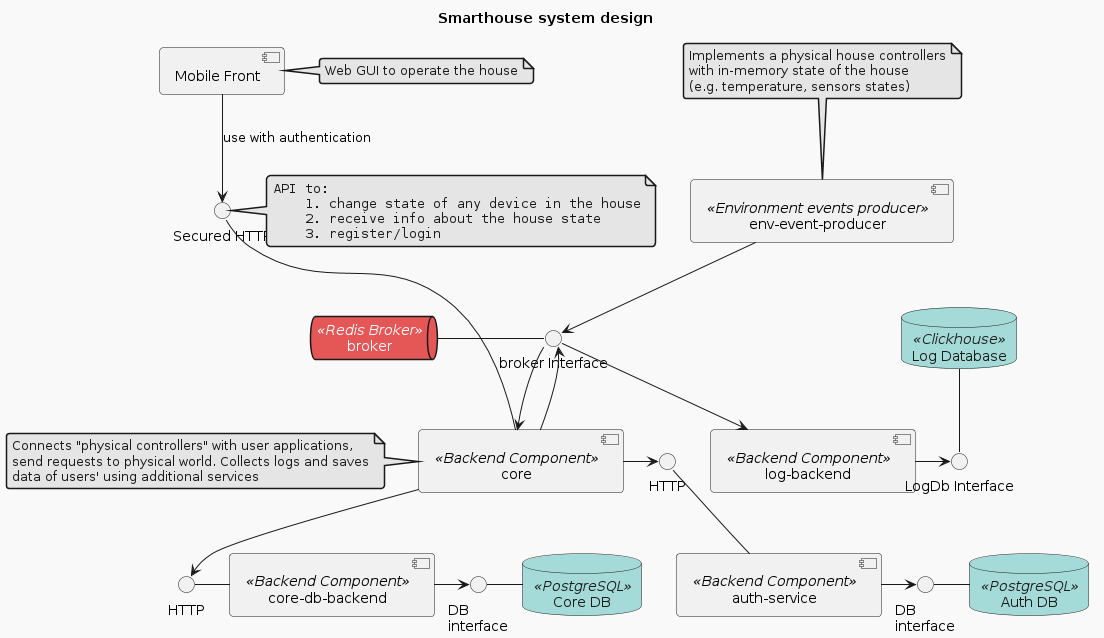
\includegraphics[height=10.5cm]{images/SmartHouse_System_Design.png}
}
\caption{Дизайн системы интеграций SmartHouse}
\end{figure}

\subsection{Диаграммы последовательности}
\begin{figure}[H]
    \centering{\vspace*{0.4cm}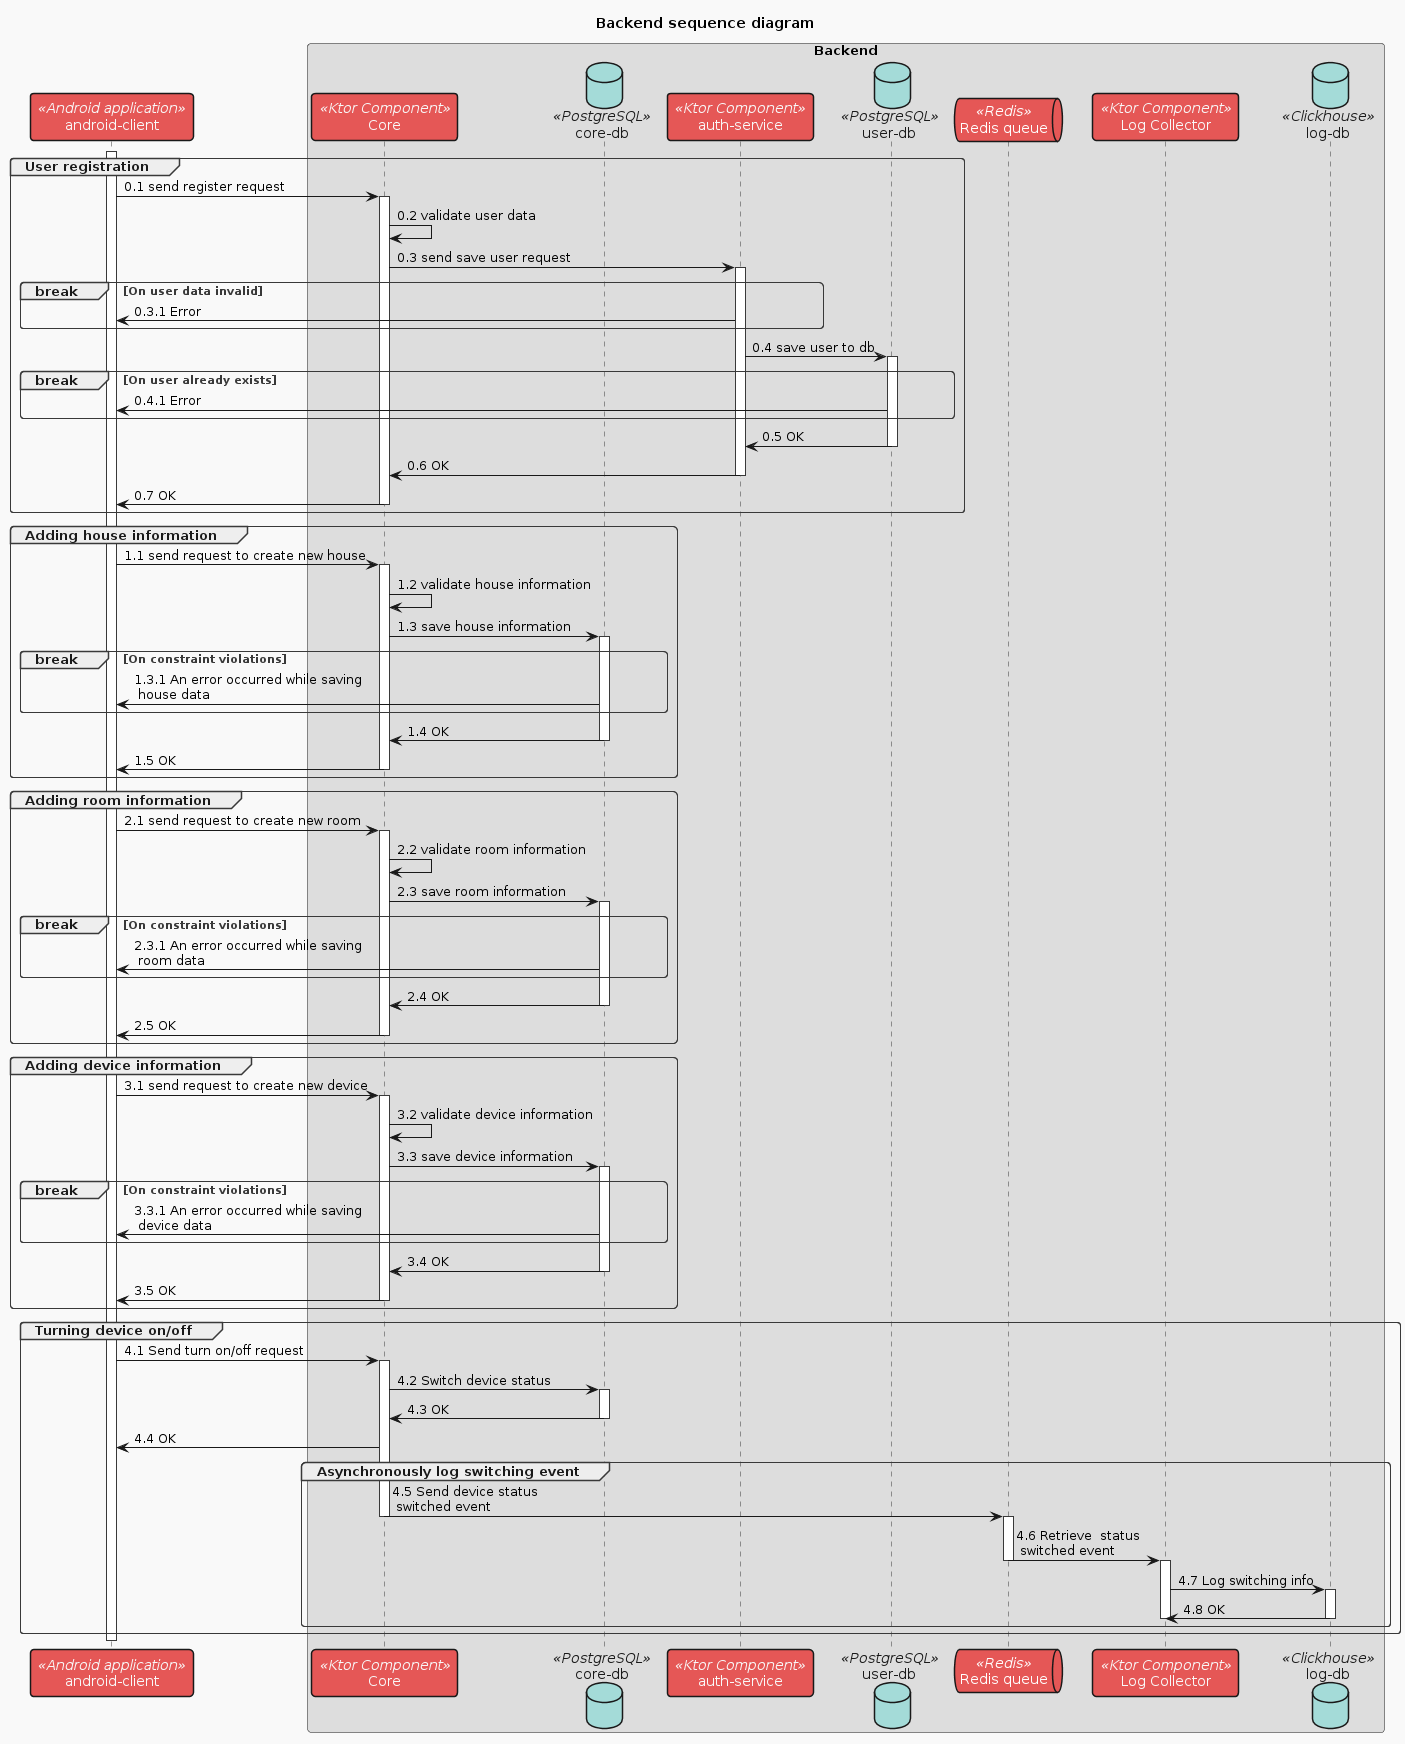
\includegraphics[height=20.5cm]{images/Smarthouse_sequence_backend.png}}
    \caption{Sequence-диаграмма backend'a}
\end{figure}

\begin{figure}[H]
    \centering{\vspace*{0.4cm}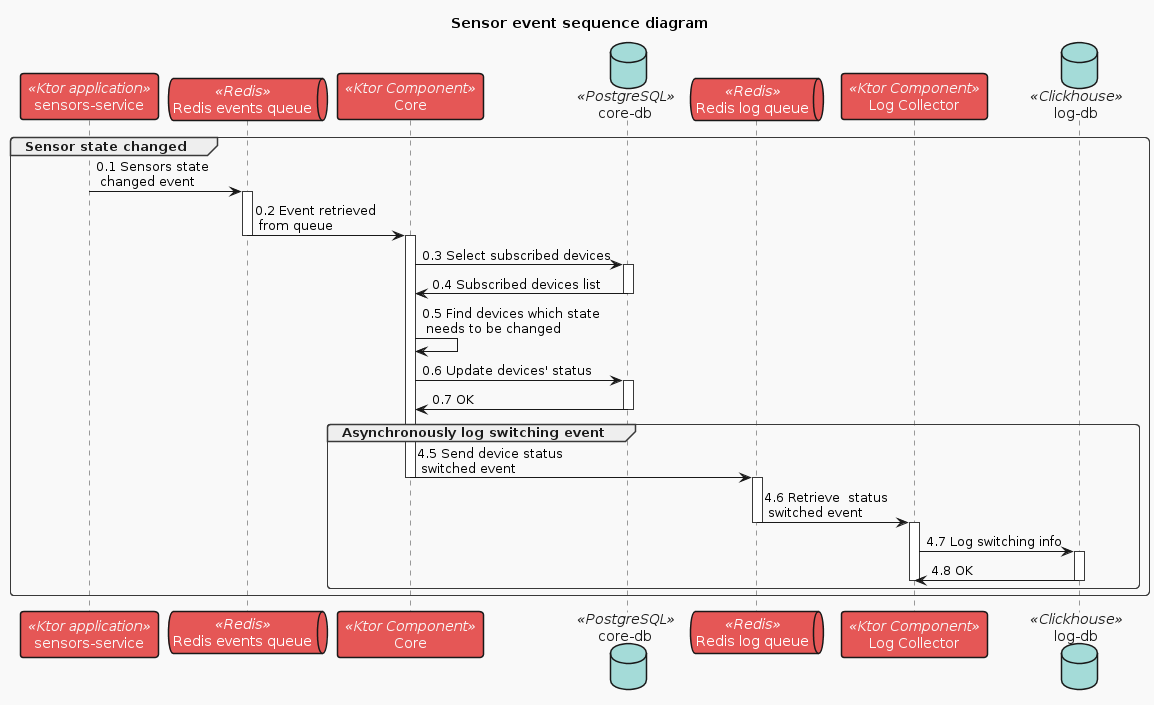
\includegraphics[height=10.5cm]{images/Smarthouse_sequence_sensore_event.png}}
    \caption{Sequence-диаграмма события с сесноров}
\end{figure}

\begin{figure}[H]
    \centering{\vspace*{0.4cm}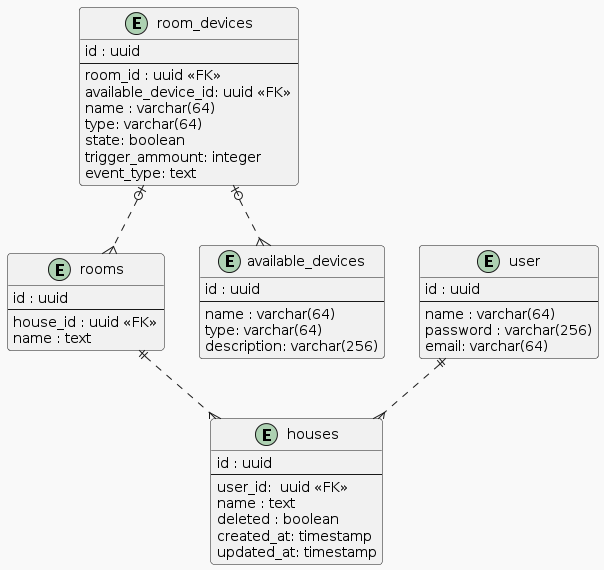
\includegraphics[height=10.5cm]{images/Smarthouse_ERD.png}}
    \caption{ERD-диаграмма сущностей в БД}
\end{figure}


\begin{figure}[H]
    \centering
    \subfigure[]{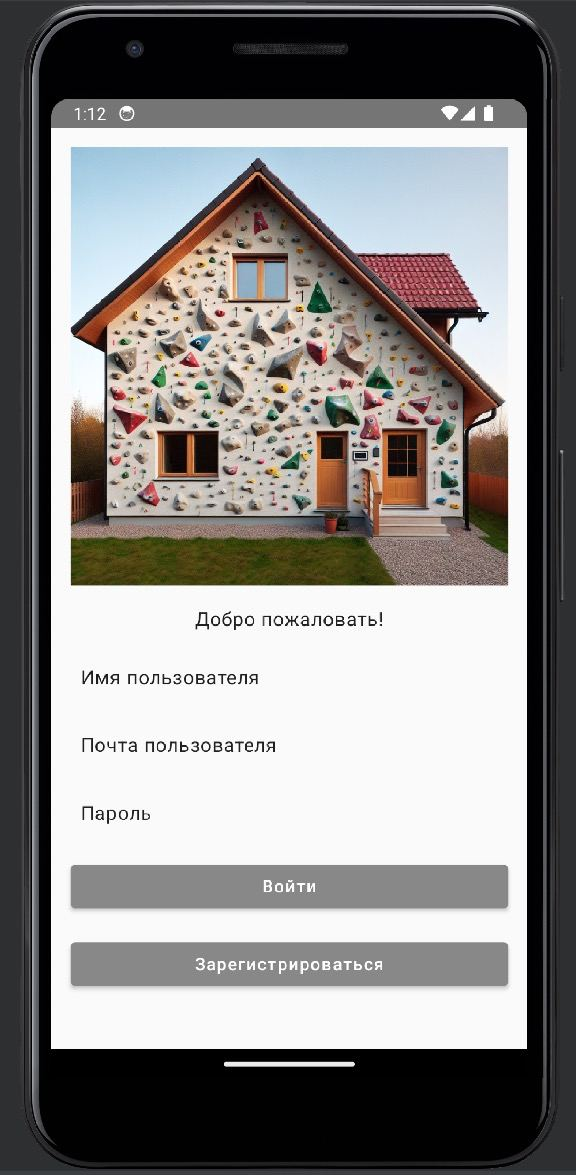
\includegraphics[height=7.5cm]{images/Smarthouse_login_page.jpg}} 
    \subfigure[]{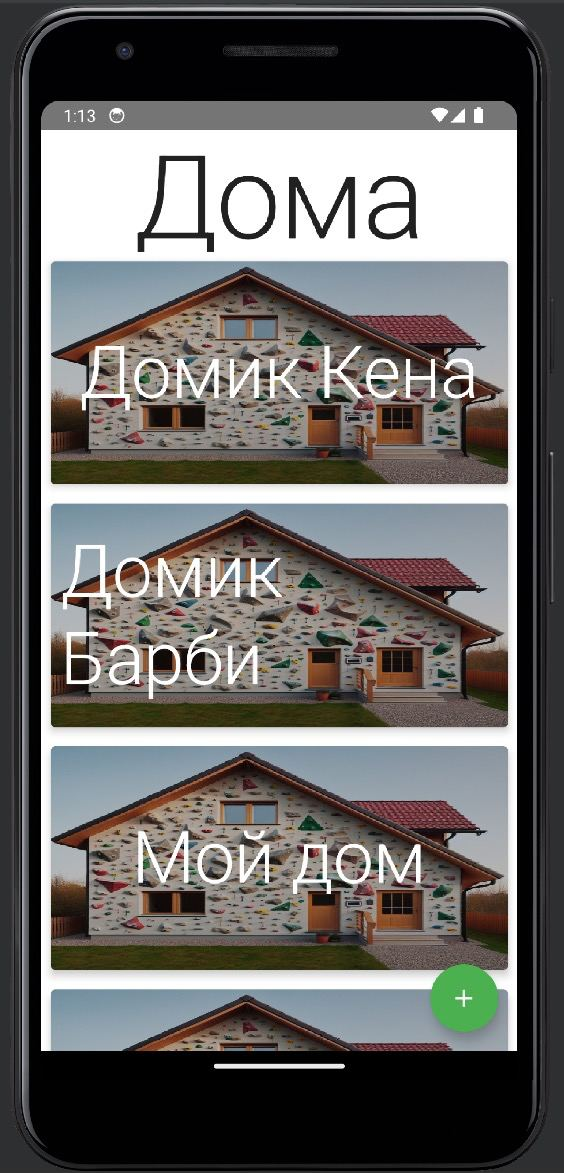
\includegraphics[height=7.5cm]{images/Smarthouse_main_page.png}} 
    \subfigure[]{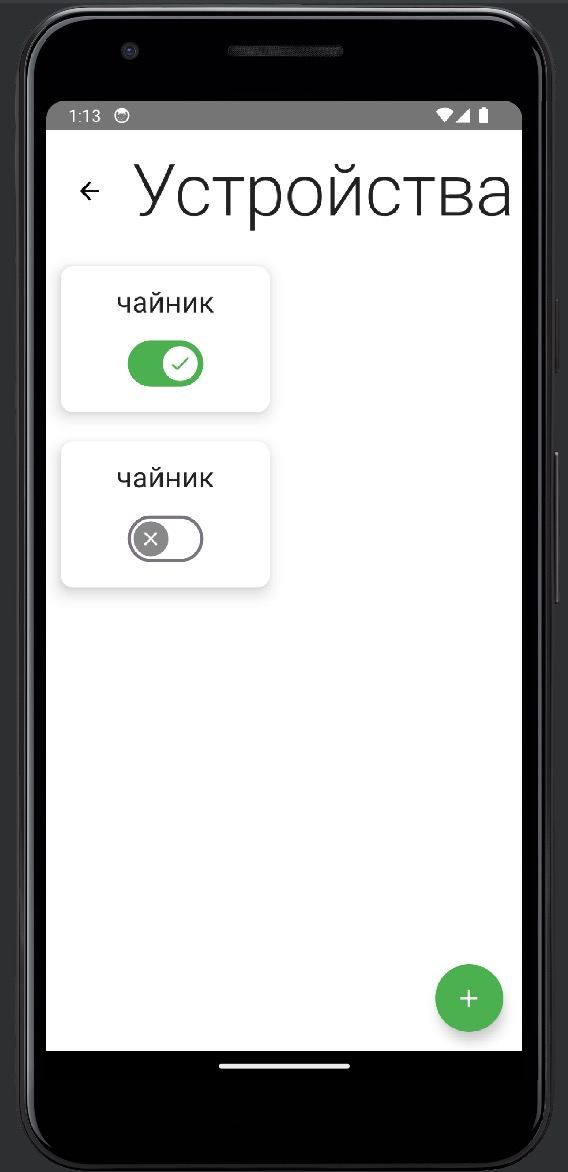
\includegraphics[height=7.5cm]{images/Smarthouse_devices_page.jpg}}
    \subfigure[]{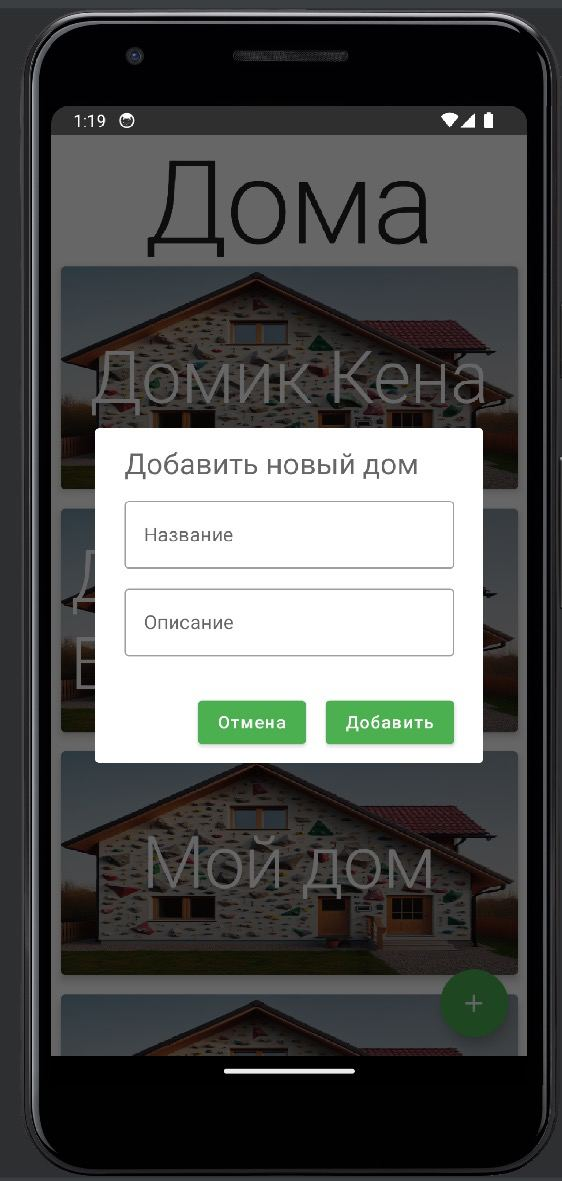
\includegraphics[height=7.5cm]{images/Smarthouse_add_item.jpg}}
    \caption{(a) Страница входа (b) Главная странца (c) Страница устройств (d) Добавление дома}
\end{figure}

\section{Используемые технологии}

\begin{enumerate}
    \item Backend:
        \begin{enumerate}
            \item Kotlin
            \item Gradle
            \item Ktor
            \item Exposed
            \item Clickhouse
            \item PostgreSQL
            \item Redis
        \end{enumerate}
    \item Frontend:
	  \begin{enumerate}
            \item Kotlin
            \item Jetpack Compose
        \end{enumerate}
\end{enumerate}

\section{Заключение}
Разработка мобильного приложения для управления умным домом представляет собой важное направление в современных технологических инновациях. Наше приложение значительно упрощает процесс контроля над домашними системами, способствуя повышению комфорта и безопасности жильцов. Ключевыми факторами для успешного выхода нашего продукта на рынок умного дома и его долгосрочного успеха станут непрерывное совершенствование функционала, адаптация к быстро меняющимся технологическим трендам, а также активное принятие и анализ обратной связи от пользователей.

\section{Список используемой литературы}

\begin{thebibliography}{}
    \bibitem{uml-link} Использование диаграммы вариантов использования UML при проектировании программного обеспечения [Электронный ресурс] / Habr. URL: \url{https://habr.com/ru/articles/566218}, свободный (дата обращения: 05.03.2024).
    \bibitem{coroutines-link} Ликбез по корутинам Kotlin [Электронный ресурс] / Habr. URL: \url{https://habr.com/ru/companies/otus/articles/766774} свободный (дата обращения: 10.03.2024)
    \bibitem{kotlin-inside-link} Kotlin: взгляд изнутри — преимущества, недостатки и особенности  [Электронный ресурс] /Habr. URL:  \url{https://habr.com/ru/articles/752450/}, свободный (дата обращения: 8.05.2023).
\end{thebibliography}

\end{document}